\documentclass[a4paper,11pt,exos]{nsi} % COMPILE WITH DRAFT
\usepackage{pifont}
\usepackage{fontawesome5}

%\pagestyle{empty}

\begin{document}
\classe{\premiere spé}
\titre{Second degré - Exercices}
\maketitle

\subsection*{Plusieurs formes pour un même polynôme}

\exo{}
Donner la forme développée des fonctions définies sur $\R$ par :
\begin{multicols}{3}
	\begin{enumerate}[label=\textbullet]
		\item 	$f(x)=(x-1)(x-2)$.
		\item 	$g(x)=(x-3)(x-4)$.
		\item	$l(x)=7(x+2)(x-5)$.
		\item 	$m(x)=-3x(x-2)$.
		\item 	$k(x)=(x-\sigma_1)(x-\sigma_2)$ \\où $\sigma_1$ et $\sigma_2$ sont deux réels.\columnbreak
	\end{enumerate}
\end{multicols}


\exo{}
Donner la forme développée des fonctions définies sur $\R$ par :
\begin{multicols}{3}
	\begin{enumerate}[label=\textbullet]
		\item 	$f(x)=(x+1)^2+1$
		\item 	$g(x)=3(x-1)^2+7$.
		\item 	$h(x)=-2(x+7)^2+2$.
		\item 	$k(x)=\left(x-\dfrac{1}{2}\right)^2+\dfrac{3}{4}$.
		\item	$l(x)=(x-\alpha)^2+\beta$\\ où $\alpha$ et $\beta$ sont deux réels.
	\end{enumerate}
\end{multicols}


\exo{}
Regrouper les expressions égales
\begin{multicols}{3}
	\begin{enumerate}[label=\textbullet]
		\item 	$2x^2-10x+12$
		\item 	$2x^2-14x+20$
		\item 	$2x^2-16x+30$
	\columnbreak
		\item 	$2(x-2)(x-5)$
		\item 	$2(x-2)(x-3)$
		\item 	$2(x-3)(x-5)$
	\columnbreak
		\item	$2\left(x-4\right)^2-2$
		\item	$2\left(x-\dfrac{7}{2}\right)^2-\dfrac{9}{2}$
		\item 	$2\left(x-\dfrac{5}{2}\right)^2-\dfrac{1}{2}$
		
	\end{enumerate}
\end{multicols}

\exo{}
Suivre le modèle suivant pour écrire les polynômes suivants sous forme canonique.\\
\textbf{\textsc{Modèle :}}
\begin{tabbing}
	$f(x)$	\=	$=x^2+2x+7\qquad\qquad\qquad\qquad\qquad$				\=	on isole les 2 premiers termes ;\\
	\>	$=\left(x^2+2x\right)+7$						\>	entre parenthèses, on voit le début \\
	\>													\>	d'une identité remarquable ;\\
	\>	$=\left(x^2+2\times x\times 1\right)+7$			\>	il manque juste le $1^2$, donc on écrit\\
	\>	$=\left(x^2+2\times x\times 1\boxed{+1^2-1^2}\right)+7$						\>	et grâce à cette astuce\\
	\>	$=\left((x+1)^2-1\right)+7$						\>	rassemblons les constantes ;\\
	\>	$=(x+1)^2+6$									\>	et voilà une forme canonique !
\end{tabbing}
\begin{multicols}{3}
	\begin{enumerate}[label=\textbullet]
		\item 	$f(x)=x^2+2x-3$.
		\item 	$g(x)=x^2+4x+1$.
		\item 	$h(x)=x^2+6x-9$.
		\item 	$k(x)=x^2-2x-1$
		\item	$l(x)=x^2-8x+10$.
		\item 	$m(x)=x^2+7x-1$.
	\end{enumerate}
\end{multicols}

\exo{- Utiliser la forme factorisée pour résoudre une inéquation liée au signe}
On considère la fonction définie sur $\R$ par $\quad f(x)=3 x^2+12x-15$
\begin{enumerate}
	\item 	Montrer que pour tout $x\in\R$ on a $\quad f(x)=3(x-1)(x+5)$.
	\item 	À l'aide d'un tableau de signes, résoudre l'inéquation $f(x)\leq 0$.
	\item 	Montrer que pour tout $x\in\R$ on a $\quad f(x)+24 = 3(x+3)(x+1)$.
	\item	Résoudre $f(x)\geqslant -24$.
\end{enumerate}

\exo{- Utiliser la forme canonique}
On considère la fonction $g$ définie sur $\R$ par $\quad g(x)=-0,5(x-4)^2+5$.

\begin{enumerate}
	\item 	Donner le tableau de variation de $g$ sur $\R$.
	\item 	Compléter le tableau de valeurs suivant : \hspace{3em}
	\begin{tabular}{|c|c|c|c|}
		\hline 
		$x$    & 4 & 6 & 8 \\ 
		\hline 
		$g(x)$ & $\quad$  & $\quad$  & $\quad$  \\ 
		\hline 
	\end{tabular}\\ 
	
	\item 	Représenter $\courbe{g}$ dans le repère ci-dessous :
	\begin{center}
		\begin{tikzpicture}[]
			\repereal{-2}{-4}{9}{6}
		\end{tikzpicture}
	\end{center}
	\item 	Résoudre graphiquement  $g(x)=0,5$.
	\item 	Retrouver ce résultat par le calcul.
\end{enumerate}


\subsection*{Des paraboles}
\exo{}
\def\xmin{-5}\def\ymin{-5}\def\xmax{5}\def\ymax{5}
\def\F{-(\x-2)*(\x-2)+3}
\def\G{-(\x+1)*(\x+1)*.5-2}
\def\H{2*(\x+1)*(\x+1)-1}
\def\K{(\x-1)*(\x-1)*.2-2}

\dleft{7.5cm}
{
	\begin{tikzpicture}[scale= .65]
		\reperevl{\xmin}{\ymin}{\xmax}{\ymax}
		\clip (\xmin,\ymin) rectangle (\xmax,\ymax);
		\draw[thick,domain=\xmin:\xmax,smooth,variable=\x] plot ({\x},{\F});
		\draw[thick,domain=\xmin:\xmax,smooth,variable=\x] plot ({\x},{\G});
		\draw[thick,domain=\xmin:\xmax,smooth,variable=\x] plot ({\x},{\H});	
		\draw[thick,domain=\xmin:\xmax,smooth,variable=\x] plot ({\x},{\K});
		\draw 	(-4,-4.5) node{$\courbe{_1}$} 
		(-4,2) node{$\courbe{_2}$}
		(1,4) node{$\courbe{_3}$}
		(4,-4) node{$\courbe{_4}$};
	\end{tikzpicture}
}
{
	Voici les expressions de quatre fonctions polynôme du second degré :
	\begin{enumerate}[label=\textbullet]
		\item 	$f(x)=\dfrac{1}{5}(x-1)^2-2$
		\item 	$g(x)=(x+1)^2-1$
		\item 	$h(x)=-\dfrac{1}{2}(x+1)^2-2$
		\item 	$k(x)=-(x-2)^2+3$
	\end{enumerate}
	Associer chaque fonction à sa courbe représentative.
}
%\vspace{0.5cm}

\exo{}
\dleft{9.5cm}
{
	Voici les expressions de quatre fonctions polynôme du second degré
	\begin{enumerate}[label=\textbullet]
		\item 	$f(x)=-\dfrac{1}{5}(x-4)(x-1)$
		\item 	$g(x)=-(x-3)(x+2)$
		\item 	$h(x)=(x+1)^2$
		\item 	$k(x)=2(x+4)(x+3)$
	\end{enumerate}
	Associer chaque fonction à sa courbe représentative.
}
{
	\def\xmin{-5}\def\ymin{-3}\def\xmax{5}\def\ymax{7}
	\def\F{-(\x-3)*(\x+2)}
	\def\G{-(\x-4)*(\x-1)*.2}
	\def\H{(\x+1)*(\x+1)}
	\def\K{(\x+4)*(\x+3)*2}
	\begin{tikzpicture}[scale=.65]
		\reperevl{\xmin}{\ymin}{\xmax}{\ymax}
		\clip (\xmin,\ymin) rectangle (\xmax,\ymax);
		\draw[thick,domain=\xmin:\xmax,smooth,variable=\x] plot ({\x},{\F});
		\draw[thick,domain=\xmin:\xmax,smooth,variable=\x] plot ({\x},{\G});
		\draw[thick,domain=\xmin:\xmax,smooth,variable=\x] plot ({\x},{\H});	
		\draw[thick,domain=\xmin:\xmax,smooth,variable=\x] plot ({\x},{\K});
		\draw 	(4.5,-1) node{$\courbe{_1}$} 
		(-4.5,3) node{$\courbe{_2}$}
		(-4,6) node{$\courbe{_3}$}
		(-3,-2) node{$\courbe{_4}$};
	\end{tikzpicture}
}
%\vspace{0.5cm}

\exo{}
\dleft{7.5cm}
{
	\def\xmin{-4}\def\ymin{-4}\def\xmax{6}\def\ymax{6}
	\def\F{(\x-2)*(\x-2)-3}
	\def\G{(\x-2)*(\x-2)*2-3}
	\def\H{(\x-2)*(\x-2)/2-3}
	\begin{tikzpicture}[scale= .65]
		\reperevl{\xmin}{\ymin}{\xmax}{\ymax}
		\clip (\xmin,\ymin) rectangle (\xmax,\ymax);
		\draw[thick,domain=\xmin:\xmax,smooth,variable=\x] plot ({\x},{\F});
		\draw[thick,dotted,domain=\xmin:\xmax,smooth,variable=\x] plot ({\x},{\G});
		\draw[thick,dashed,domain=\xmin:\xmax,smooth,variable=\x] plot ({\x},{\H});	
		
	\end{tikzpicture}
}
{
	Voici les expressions de trois fonctions polynôme du second degré
	\begin{enumerate}[label=\textbullet]
		\item 	$f(x)=\dfrac{1}{2}(x-2)^2-3$
		\item 	$g(x)=2(x-2)^2-3$
		\item 	$h(x)=(x-2)^2-3$
	\end{enumerate}
	Associer chaque fonction à sa courbe représentative.
}
%\vspace{0.5cm}

\exo{}
Résoudre dans $\R$ les équations suivantes : 
\begin{multicols}{2}
	\begin{enumerate}
		\item 	$\left(x+1\right)^2-3=0$
		\item 	$\left(x-7\right)^2-8=0$
		\item	$2(x+3)^2-50=0$
		\item	$3(x-2)^2+7=0$
	\end{enumerate}
\end{multicols}


\exo{}
$f$ est une fonction polynôme du second degré.\\
Quelle est la forme la plus adaptée (développée, factorisée ou canonique) permettant de répondre aux questions suivantes ?
\begin{enumerate}
	\item 	Déterminer l'image de 0 par $f$.
	\item 	Démontrer le sens de variation de $f$.
	\item	Résoudre $\quad f(x)=0$.
	\item	Résoudre $\quad	f(x)=c$.
	\item	Déterminer l'extremum de $f$.
\end{enumerate}


\exo{}
$f$ est une fonction polynôme du second degré.\\
On donne les informations suivantes :
\begin{enumerate}[label=\textbullet]
	\item 	Les antécédents de 0 par $f$ sont $-2$ et $3$.
	\item 	L'image de 4 par $f$ est $-5$.	
\end{enumerate}
Déterminer une expression de $f$ en fonction de $x$.



\exo{}
L'unité est le centimètre.\\
AB=10 et M est un point de [AB].\\
AMNP est un carré, MBCQ est un rectangle et BC=4.

\begin{center}
	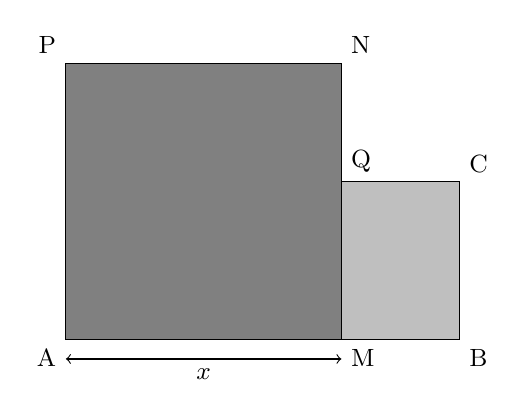
\begin{tikzpicture}[scale=.5]
		\draw[fill=gray](0,0) rectangle (7,7);
		\draw[fill=gray!50](7,0) rectangle (10,4);
		\draw 	(0,0) node[below left]{\small A} 
		(7,0)node[below right]{\small M} 
		(10,0)node[below right]{\small B}
		(10,4)node[above right]{\small C}
		(7,4) node[above right]{\small Q}
		(7,7) node[above right]{\small N}
		(0,7) node[above left]{\small P};
		\draw[<->] (0,-.5) -- node[midway,below]{\small $x$}(7,-.5); 
	\end{tikzpicture}
\end{center}

\textbf{\boldmath On pose $AM=x$.\\
	On note $f(x)$ la somme des aires de AMNP et MBCQ  en fonction de $x$.}

\begin{enumerate}
	\item 	Quel est l'ensemble de définition de $f$ ? 
	\item 	Faire une figure pour $x=3$.
	\item 	Quelle est, en fonction de $x$, l'aire du carré AMNP ?
	\item 	Que vaut, en fonction de $x$, la distance MB ?
	\item 	En déduire l'aire du rectangle $MBCQ$.
	\item 	Montrer que pour tout $x\in\mathcal{D}_f$ on a $\quad f(x)=x^2-4x+40$.
	\item 	Montrer que pour tout $x\in\mathcal{D}_f$ on a $\quad f(x)=(x-2)^2+36$.
	\item 	Donner le tableau de variation de $f$ sur $\mathcal{D}_f$.	\item	Pour quelle valeur de $x$ la somme des aires est-elle minimale ?
	\item 	Y a-t-il des valeurs de $x$ pour lesquelles la somme des aires vaut 85cm$^2$ ?
	\item 	Représenter $\courbe{f}$ sur la calculatrice, avec une fenêtre convenable.
\end{enumerate}


\subsection*{Forme factorisée et racines d'un polynôme}

\exo{}
Donner les formes factorisées (si elles existent) des fonctions définies sur $\R$ par :
\begin{multicols}{3}
	\begin{enumerate}[label=\textbullet]
		\item 	$f(x)=2x^2-5x+3$
		\item 	$g(x)=3x^2+2x+4$
		\item 	$h(x)=x^2+x+1$
		\item 	$j(x)=3x^2-2x+\dfrac{1}{3}$
		\item 	$k(x)=-3x^2+x+1$
		\item 	$l(x)=4x^2-4x+15$
	\end{enumerate}
\end{multicols}


\exo{}
Résoudre les équations suivantes dans $\R$ :
\begin{multicols}{3}
	\begin{enumerate}
		\item 	$7x^2+5x+1=0$
		\item 	$0,5x^2+2,5x+15=0$
		\item 	$2x^2-7x+3=0$
		\item $15 x^{2}-8 x-12=0$
		\item $x^2-8=0$
		\item $2(x^2+x)=-3$
		\item $15x^2-6x+\dfrac{3}{5}=0$
		\item $3x^2-2x=0$
		\item $x^2+\sqrt{2}x-4=0$
		\item $12x^2+8x-15=0$
		\item $2+9x^2=0$
		\item $20x^2-8x+\dfrac{4}{5}=0$
		\item $2(x^2-x)=-5$
		\item $5x^2=x$
		\item $x^2+2\sqrt{3}x-9=0$
	\end{enumerate}
\end{multicols}

\exo{}
Léna a écrit le script Python ci-dessous :
\begin{pyc}
    \begin{minted}{python}
a = float(input("entrez a"))
b = float(input("entrez b"))
c = float(input("entrez c"))
delta = b ** 2 - 4 * a * c
if delta > 0 :
    print(2)
elif delta == 0 :
    print(1)
else :
    print(0)        
    \end{minted}
\end{pyc}
\begin{enumerate}
	\item 	À quoi correspond le nombre affiché par ce script lorsqu'on entre les valeurs 2, 5 et 1 ?
	\item 	Proposer un script en Python qui permet d'afficher les éventuelles racines réelles d'un polynôme du second degré à partir de ses coefficients.\\
	\textit{Aide : En Python, on calcule la racine carrée de $x$ en tapant }\pythoninline{sqrt(x)}.\\
	Tu peux saisir ce script dans ta calculatrice, et l'utiliser pour vérifier tes calculs.
\end{enumerate}


\exo{ Somme et produit des racines d'un polynôme du second degré}
Soient $x_1$ et $x_2$ deux nombres réels.\\
On se donne une fonction polynôme du second degré $f$ définie sur $\R$ par : $$ f(x)=(x-x_1)(x-x_2).$$
\begin{enumerate}
	\item 	Que représentent $x_1$ et $x_2$ pour $f$ ?
	\item 	Montrer que la forme développée de $f$ est donnée par $\quad f(x)=x^2-sx+p\quad$ avec $s$ et $p$ deux réels.\\
	Que représentent les réels $s$ et $p$ pour $f$ ?
	\item	\textbf{Application :}
	\begin{enumalph}
		\item 	Déterminer deux réels dont la somme est $-24$ et le produit est $135$.
		\item 	Déterminer deux réels dont la somme est $\dfrac{5}{2}$ et le produit est $-\dfrac{3}{2}$.
	\end{enumalph} 
\end{enumerate}

\subsection*{Inéquations du second degré}

\exo{}
Résoudre les inéquations suivantes :
\begin{multicols}{3}
    	\begin{enumerate}
		\item 	$2x^2-3x-2\geqslant 0$
		\item	$5x^2-6x<0$
		\item 	$-3x^2+30x-75>0$
		\item 	$-x^2+6x-9\leqslant 0$	
		\item 	$-2x^2+3x-1\leqslant 0$
	\end{enumerate}
\end{multicols}

\subsection*{Mise en équations}

\exo{}
	La longueur d'un rectangle surpasse sa largeur de 7 cm. Sa surface est de 228 cm$^2$. Quelles sont ses dimensions ?
	
	\exo{}
	On doublera la surface d'un jardin rectangulaire $16\times 24$ m si on l'entoure d'une bande de $x$ m de large. Déterminer $x$.\\
	
	\exo{}
	Un drapeau d'inspiration danoise a pour dimensions 3 m sur 2 m, la croix, blanche sur fond rouge, est composée de deux bandes de même largeur.
	\begin{center}
		\def\larg{.3486}	
		\begin{tikzpicture}
			\draw[thick,fill=red] (0,0) rectangle (3,2);
			\draw[white, fill=white] (1-\larg,0) rectangle (1+\larg,2);
			\draw [white, fill=white](0,1-\larg) rectangle (3,1+\larg);
			\draw (0,0) rectangle (3,2);
		\end{tikzpicture}
	\end{center}	
	Quelle largeur doivent avoir ces bandes pour que l'aire de la croix soit égale à celle du fond rouge ?
	
	
	\exo{$^\bigstar$}
	Un père et son fils travaillent chez le même entrepreneur. Après un certain nombre d'heures de travail, le père reçoit 500 €.\\
	Le fils, qui a travaillé 5 heures de moins et dont le salaire horaire est inférieur de 8 € à celui de son père, ne reçoit que 240 €.\\
	Le but de l'exercice est de déterminer le salaire horaire de chacun et le nombre d'heures qu'ils ont travaillé.\\[.5em]
	On appelle $x$ le salaire horaire du père et $n$ le nombre d'heures effectuées par le père.
	
	\begin{enumerate}
		\item 	Exprimer $n$ en fonction de $x$.
		\item 	Exprimer le salaire horaire du fils en fonction de $x$.
		\item 	Exprimer le nombre d'heures effectuées par le fils en fonction de $x$.
		\item 	Montrer que l'équation du problème est $\quad \left(x-8\right)\left(\dfrac{500}{x}-5\right)=240$.
		\item	Résoudre cette équation.
		\item 	Sachant que le père et le fils on travaillé un nombre \textbf{entier} d'heures, déterminer le salaire horaire de chacun et le 
		nombre d'heures qu'ils ont travaillées.
	\end{enumerate}

\subsection*{Pour approfondir}

\exo{}
Résoudre dans $\R$ les équations suivantes :
\begin{multicols}{2}
	\begin{enumerate}
		\item 	$\dfrac{x-1}{2x-5}=\dfrac{x+1}{x-1}$
		\item 	$\dfrac{2x^2-3x-2}{x-2}=x+1$
	\end{enumerate}
\end{multicols}


\exo{}
Résoudre dans $\R$ les inéquations suivantes :
\begin{multicols}{2}	
	\begin{enumerate}
		\item 	$\dfrac{x^2}{x+2}>1$
		\item 	$\dfrac{-3x+1}{2-x}\leqslant\dfrac{-4x+5}{x+3}$
	\end{enumerate}
\end{multicols}



\exo{}
Pour quelle(s) valeur(s) du réel $a$ l'équation $\quad x^2+ax+1=0 \quad$  admet-elle deux racines distinctes dans $\R$ ?

\exo{ \'Equation bicarré}
On veut résoudre dans $\R$ l'équation  $$(E):\qquad x^4-3x^2-4=0$$
\begin{enumerate}
	\item 	Poser $X=x^2$ et résoudre l'équation obtenue en remplaçant $x^2$ par $X$ dans $(E)$.
	\item 	En déduire les solutions de $(E)$.
\end{enumerate}

\end{document}